\section{Designing the System}

Using diagrams and charts that will help you to understand the structure and relationships in the system and how it was planned to be from the beginning. 

The Core is the heart of Drupal, it represents a standard release of Drupal which encloses fundamental features to build a basic site. As you can see Drupal Core encircle Themes, User Permissions, Blocks, Modules and Nodes.

\begin{figure}[H]
\centering
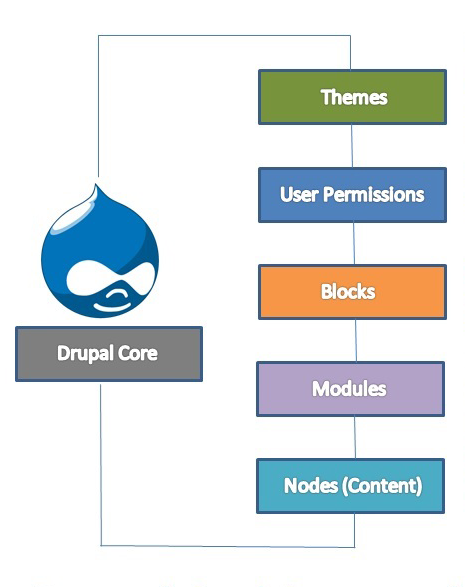
\includegraphics[width=14cm]{Chapter2/drupal_architectural_layers.png}
\caption{Drupal Architecture Layers}
\label{fig:drupal_architectural_layers}
\end{figure}

\subsection{Themes}
A theme defines your site’s user interface (UI). It is a collection of files that are interpreted by a Theme Engine to create the desired visual output. Here is used Javascript and jQuery to code visual elements. To understand how Drupal works, you need to understand Drupal's page serving mechanism.

\begin{figure}[H]
\centering
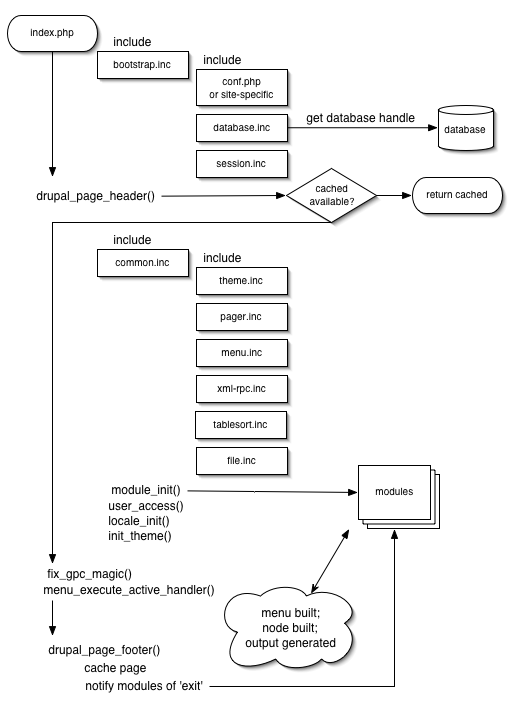
\includegraphics[width=14cm]{Chapter2/drupal_page_serving_mechanism.png}
\caption{Drupal Page Serving Mechanism}
\label{fig:drupal_page_serving_mechanism}
\end{figure}

In short, all the calls/urls/requests are served by index.php which loads Drupal by including various include files/modules and then calling the appropriate function, defined in module, to serve the request/url.

\subsubsection{The Bootstrap Process}

Drupal bootstraps itself on every request by going through a series of bootstrap phases. These phases are defined in bootstrap.inc and proceed as described in the following sections.

\subsubsection{Initialize Configuration}

This phase populates Drupal’s internal configuration array and establishes the base URL (\$base\_url) of the site. The settings.php file is parsed via include\_once(), and any variable or string overrides established there are applied.

\subsubsection{Early Page Cache}

In situations requiring a high level of scalability, a caching system may need to be invoked before a database connection is even attempted. The early page cache phase lets you include (with include()) a PHP file containing a function called page\_cache\_fastpath(), which takes over and returns content to the browser. The early page cache is enabled by setting the page\_cache\_fastpath variable to TRUE, and the file to be included is defined by setting the cache\_inc variable to the file’s path. See the chapter on caching for an example.

\subsubsection{Initialize Database}

During the database phase, the type of database is determined, and an initial connection is made that will be used for database queries.

\subsubsection{Hostname/IP-Based Access Control}

Drupal allows the banning of hosts on a per-hostname/IP address basis. In the access control phase, a quick check is made to see if the request is coming from a banned host; if so, access is denied.

\subsubsection{Initialize Session Handling}

Drupal takes advantage of PHP’s built-in session handling but overrides some of the handlers with its own to implement database-backed session handling. Sessions are initialized or reestablished in the session phase. The global \$user object representing the current user is also initialized here, though for efficiency not all properties are available (they are added by an explicit call to the user\_load() function when needed).

\subsubsection{Late Page Cache}

In the late page cache phase, Drupal loads enough supporting code to determine whether or not to serve a page from the page cache. This includes merging settings from the database into the array that was created during the initialize configuration phase and loading or parsing module code. If the session indicates that the request was issued by an anonymous user and page caching is enabled, the page is returned from the cache and execution stops.

\subsubsection{Language Determination}

At the language determination phase, Drupal’s multilingual support is initialized and a decision is made as to which language will be used to serve the current page based on site and user settings. Drupal supports several alternatives for determining language support, such as path prefix and domain-level language negotiation.

\subsubsection{Path}

At the path phase, code that handles paths and path aliasing is loaded. This phase enables human-readable URLs to be resolved and handles internal Drupal path caching and lookups.

\subsubsection{Full}

This phase completes the bootstrap process by loading a library of common functions, theme support, and support for callback mapping, file handling, Unicode, PHP image toolkits, form creation and processing, mail handling, automatically sortable tables, and result set paging. Drupal’s custom error handler is set, and all enabled modules are loaded. Finally, Drupal fires the init hook, so that modules have an opportunity to be notified before official processing of the request begins.

Once Drupal has completed bootstrapping, all components of the framework are available. It is time to take the browser’s request and hand it off to the PHP function that will handle it. The mapping between URLs and functions that handle them is accomplished using a callback registry that takes care of both URL mapping and access control. Modules register their callbacks using the menu hook (for more details, see Chapter 4).

When Drupal has determined that there exists a callback to which the URL of the browser request successfully maps and that the user has permission to access that callback, control is handed to the callback function.

\subsubsection{Processing a Request}

The callback function does whatever work is required to process and accumulate data needed to fulfill the request. For example, if a request for content such as http:\/\/example.com\/?q=node\/3 is received, the URL is mapped to the function node\_page\_view() in node.module. Further processing will retrieve the data for that node from the database and put it into a data structure. Then, it’s time for theming.

\subsubsection{Theming the Data}

Theming involves transforming the data that has been retrieved, manipulated, or created into HTML (or XML or other output format). Drupal will use the theme the administrator has selected to give the web page the correct look and feel. The resulting output is then sent to the web browser.

\subsection{User Permissions - Use Case Model}

Giving rights to right people is important because usually non technical people such as content managers are messing in the site trying to do what they do not know. Control what users do on your website by assigning them User Permissions to access features on your site. User Permissions provides an interface for giving additional permissions to individual users without the need to assign them to a special role. When this module is enabled, users with the 'administer permissions' permission can access the 'User Permissions' tab on each user's account.

\begin{figure}[H]
\centering
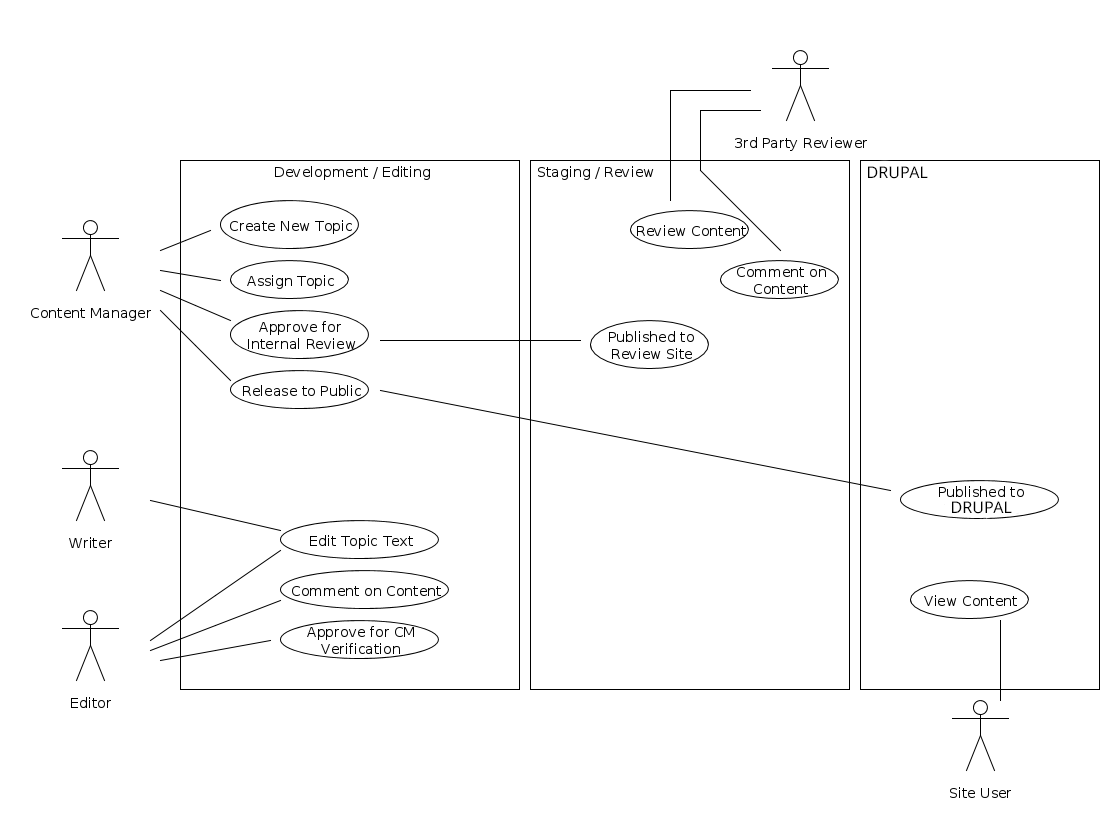
\includegraphics[width=14cm]{Chapter2/use_case.png}
\caption{Use Case}
\label{fig:use_case}
\end{figure}

One of the great features of Drupal is the ability to control how and what people can access on your site. You can set permissions for these users to define who can do what for Drupal core features and contributed modules. For example, you probably won't want casual visitors to edit your homepage. However, the site owner or trusted user should be able to do so. 

Drupal allows you to setup any number of different kinds of users or \'Roles\'. Many websites have editor and site administrator roles; editors to make content updates and site admins to install new modules and make larger configuration changes.

\subsection{Blocks}

A block represents the boxes that appear in a Drupal site. Configure blocks to customize menus, footers and other widgets type sections. Blocks in Drupal 8 are actually made up of two separate API structures to create a user experience similar to what Drupal has maintained in past iterations. These two APIs are the Block Plugin API, which is a stand-alone reusable API and the Block Entity API which is a Drupal 8 specific use case of block placement and visibility control.
	
Blocks are made available to your site most commonly by enabling core or contributed modules. Once created, a Block can be modified to adjust its appearance, shape, size and position - or which Website pages it appears on. For example, enabling the core Poll module makes the "Most Recent Polls" block available for you to place in a region. Also note that some modules provide multiple blocks when enabled, others may not define new blocks.

\subsection{Modules - Sequence Model}

A Module adds functionality to Drupal’s core. Hooks are used to ensure modules interact smoothly with the core.

\begin{figure}[H]
\centering
\includegraphics[width=14cm]{Chapter2/sequence_diagram.png}
\caption{Sequence Diagram}
\label{fig:sequence_diagram}
\end{figure}

In the previous sequence diagram represents a list of Drupal Events matching specified criteria and ask the user to select one or several events by NID. It will then proceed to check for collision with existing Google Calendar entries. It would be nice to figure out some kind of unique key that crossed the SQL and Google barrier.


\subsection{Nodes}
Content on Drupal sites are represented by Nodes. A node can take the avatar of any content type a web page, poll, blog entry, form or newsletter. In reality this would probably have several other states but for the sake of this example.

\subsubsection{State Machine Model}

A state machine is defined by the list of possible states and the event/condition that triggers each transition. In this simple ticket example the states are in progress, approval, and finished. The transitions are completed, rejected, accepted. 

\begin{figure}[H]
\centering
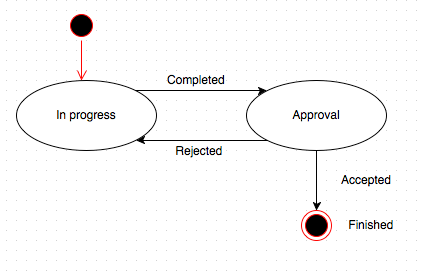
\includegraphics[width=14cm]{Chapter2/state.png}
\caption{State}
\label{fig:state}
\end{figure}

Drawing out a state machine diagram to model this kinds of problems can be really useful to help identify any edge case scenarios you may not have thought of, and capture them early in the design process. It also shows you exactly what you need to test further along in the site build.
	
As with anything in Drupal there are several ways to achieve this functionality, in fact there’s even a State Machine module, but that relies on creating custom plugins. Workbench Moderation and various other workflow modules include a state machine implementation for a specific purpose. In Drupal we’ll be using a simple list field to store the list of possible states for the node.

In Drupal 7 we need a module to help us do this. In this case we are adding a field that will never be directly edited by the user so we just deny access to edit that field using the Field Permissions module.

For the simple ticket example, we have 3 states. So use an integer list field with the following allowed values:

\begin{itemize}
\item In progress
\item Awaiting approval
\item Finished
\end{itemize}

State machine was defined by the set of possible states implemented by list field, and a set of transitions. These transitions can be implemented using the Rules Link module. Using the Rules Link module you can add a button to the ticket node which manipulates the state value preventing the user from actually editing the value in the state field directly, and thus enforcing the workflow defined in our state machine. Each 'Rules link' is configured in two parts. First you define the conditions for when the link should be visible using standard Rules conditions. Secondly, you use the rules reaction to set the value of the state field to the new value and perform any other actions that you want as a side effect of the transition.

\subsubsection{Class Model}

The taxonomy mechanism is the heart of what makes Drupal so different from most other content management systems. But experience in the drupal support channel shows it is not always well understood.

\begin{figure}[H]
\centering
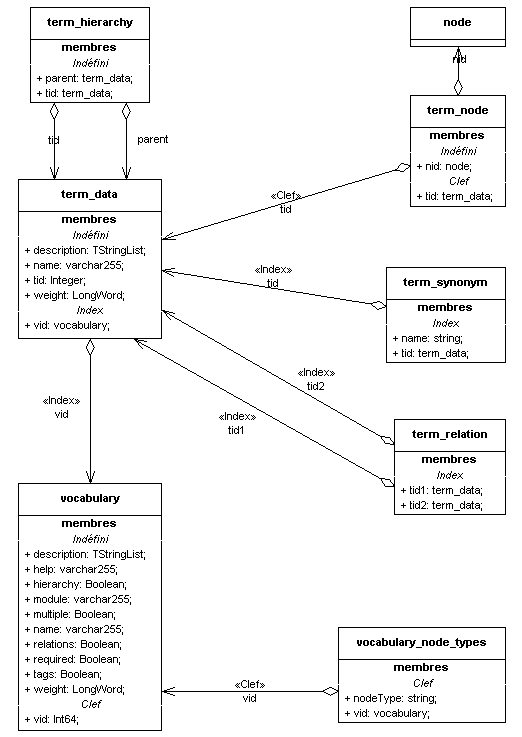
\includegraphics[width=14cm]{Chapter2/class_diagram.png}
\caption{Class Diagram}
\label{fig:class_diagram}
\end{figure}

First things first, although the service provided by the taxonomy mechanism is simple, the implementation requires no less than six tables for basic features:

The main table is term\_data. This is where the terms used for classification are defined. Every term is given a unique term identifier, or tid.
The second most important table is vocabulary. Each of the terms in term\_data belongs in exactly one vocabulary, to which it is linked by the vid column.
For vocabularies allowing it, term hierarchy is defined, obviously enough, in term\_hierarchy, in which each tid has one row for each of its parent tids, or one row with parent tid 0.
Terms are mostly used to classify the basic unit of content in Drupal, the node. This is the purpose of the term\_nodetable, which implements the term\/node relationship. Note that they can be used for other purposes like user classification.
Synonyms are handled through the use of the term\_synonym table, in which each row links to an existing tid and defines a new name for it.
For vocabularies in which this option has been enabled, the term\_relation allows for the inter-linking of terms: each row defines a pair of tid values as describing related terms.
Drupal allows vocabularies to be limited to some node types. This is implemented by the vocabulary\_node\_types lookup table

There is an implied integrity relationship : node\/type must match vocabulary\_node\_types\/nodeType for every instance of term\_node\/tid. This is currently implemented in code by drupal modules. In the current implementation each tid will also have at least one row in this table, with parent = 0, to show it is a \"root\" node. It may have more than one parent, which prevents replacing the term\_hierarchy table by just a parent column in the term\_datatable. Since this is essentially an implementation artefact that costs significant data space, it does not seem poised to remain in place for very long.

As questions on the support channel suggest, the use of drupal categories, as implemented by the taxonomy module may not be guided enough: in case where the user wants additional code to prevent terms in one category to be used on a node along with other terms from another category on the same node. In most cases, this points to an information architecture problem at a higher level: if terms are mutually dependent, like these terms that had to be exclusive, then they belong in the same classification axis, meaning the same vocabulary.

This is where the hierarchical nature of Drupal classifications comes in handy: instead of defining a set of specialized vocabularies with dependence on other vocabularies, all it takes is for one to define a hierarchical vocabulary, within which specialized subtrees will be implemented as children of higher level terms, thus ensuring mutual exclusion. In short, if there is one only word to remember when designing an information taxonomy, or in layman's terms when configuring categories on Drupal, this word is orthogonality. Proper orthogonal category design will often save a lot of time implementing case-specific rules in code.
Although the taxonomy system in Drupal is geared towards use in nodes, it can be put to other uses. As a proof of concept, Karoly Negyesi has created the user's tag module enabling the use of taxonomies on users. Use your favorite search engine to query for drupal user's tag for the current URL. This module uses a term\_datauser, similar in purpose to the term\_node table in regular taxonomy use. Note that this is NOT supported code, or even contributed code, and as such should not be used on a production system unless you are ready to maintain it or have it maintained.


% proiectarea sistemului ( se recomandă 20-30 pagini, acest capitol include descrierea metodei de proiectare, proiectarea după metoda aleasă descrisă detaliat);
